\definecolor{ptten}{RGB}{0,0,0}
\definecolor{ptsixgefour}{RGB}{0,114,178}
\definecolor{ptfivegefive}{RGB}{213,94,0}
\definecolor{ptfourgesix}{RGB}{0,158,115}

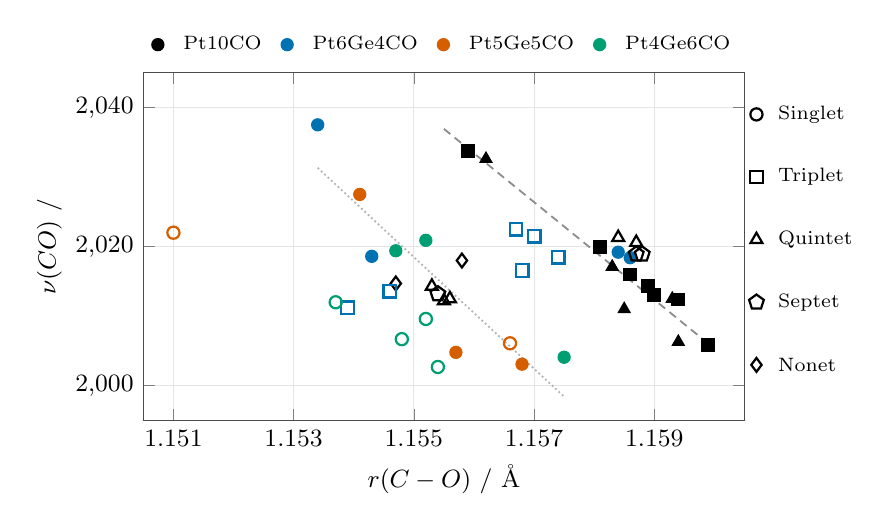
\begin{tikzpicture}
\begin{axis}[
  width=0.76\linewidth,
  height=6.0cm,
  xmin=1.1505, xmax=1.1605,
  ymin=1995, ymax=2045,
  xlabel={$r(\ce{C-O})$ / \AA},
  ylabel={$\nu(\ce{CO})$ / \si{\per\centi\metre}},
  ylabel style={yshift=-2pt},
  xtick={1.151,1.153,1.155,1.157,1.159},
  xticklabel style={/pgf/number format/fixed,/pgf/number format/precision=3},
  ytick={2000,2020,2040},
  tick label style={font=\small},
  label style={font=\small},
  grid=major,
  grid style={gray!20},
  axis line style={black!70},
  clip=false,
  legend style={at={(0.5,1.03)},anchor=south,draw=none,inner sep=1pt,
    font=\scriptsize,legend columns=4,column sep=5pt}
]
\addlegendimage{only marks,mark=*,mark size=2.2pt,ptten}
\addlegendentry{\ce{Pt10CO}}
\addlegendimage{only marks,mark=*,mark size=2.2pt,ptsixgefour}
\addlegendentry{\ce{Pt6Ge4CO}}
\addlegendimage{only marks,mark=*,mark size=2.2pt,ptfivegefive}
\addlegendentry{\ce{Pt5Ge5CO}}
\addlegendimage{only marks,mark=*,mark size=2.2pt,ptfourgesix}
\addlegendentry{\ce{Pt4Ge6CO}}
% Visual guides for the filled crossed-parent data sets only; no regression is implied.
\addplot[black!45,densely dashed,line width=0.65pt]
  coordinates {(1.15550,2036.92) (1.16000,2005.35)};
\addplot[gray!60,densely dotted,line width=0.65pt]
  coordinates {(1.15340,2031.32) (1.15750,1998.44)};
% Filled symbols: crossed-parent models.
\addplot[only marks,mark=square*,mark size=2.3pt,ptten] coordinates {
 (1.1581,2020.0) (1.1594,2012.4) (1.1589,2014.3) (1.1590,2013.0)
 (1.1599,2005.9) (1.1586,2016.0) (1.1559,2033.7)};
\addplot[only marks,mark=triangle*,mark size=2.5pt,ptten] coordinates {
 (1.1593,2012.5) (1.1583,2017.1) (1.1562,2032.6) (1.1585,2011.0)
 (1.1594,2006.3)};
\addplot[only marks,mark=*,mark size=2.2pt,ptsixgefour] coordinates {
 (1.1584,2019.2) (1.1534,2037.5) (1.1586,2018.4) (1.1543,2018.6)};
\addplot[only marks,mark=*,mark size=2.2pt,ptfivegefive] coordinates {
 (1.1568,2003.1) (1.1541,2027.5) (1.1557,2004.8)};
\addplot[only marks,mark=*,mark size=2.2pt,ptfourgesix] coordinates {
 (1.1547,2019.4) (1.1552,2020.9) (1.1575,2004.1)};
% Open symbols: models initiated from the global-minimum parent.
\addplot[only marks,mark=triangle,mark size=2.5pt,ptten,
  mark options={fill=white,draw=ptten,line width=0.8pt}] coordinates {
 (1.1584,2021.3) (1.1587,2020.6) (1.1553,2014.3) (1.1556,2012.5)
 (1.1555,2012.2)};
\addplot[only marks,mark=pentagon,mark size=2.8pt,ptten,
  mark options={fill=white,draw=ptten,line width=0.8pt}] coordinates {
 (1.1587,2018.9) (1.1588,2018.9) (1.1554,2013.2)};
\addplot[only marks,mark=diamond,mark size=2.5pt,ptten,
  mark options={fill=white,draw=ptten,line width=0.8pt}] coordinates {
 (1.1558,2018.0) (1.1547,2014.7)};
\addplot[only marks,mark=square,mark size=2.3pt,ptsixgefour,
  mark options={fill=white,draw=ptsixgefour,line width=0.8pt}] coordinates {
 (1.1574,2018.5) (1.1567,2022.5) (1.1568,2016.6) (1.1570,2021.5)
 (1.1539,2011.2) (1.1546,2013.6)};
\addplot[only marks,mark=o,mark size=2.2pt,ptfivegefive,
  mark options={fill=white,draw=ptfivegefive,line width=0.8pt}] coordinates {
 (1.1566,2006.1) (1.1510,2022.0)};
\addplot[only marks,mark=o,mark size=2.2pt,ptfourgesix,
  mark options={fill=white,draw=ptfourgesix,line width=0.8pt}] coordinates {
 (1.1552,2009.6) (1.1537,2012.0) (1.1548,2006.7) (1.1554,2002.7)};
% Symbol key: fill is reserved for the structural-parent distinction.
\addplot[only marks,mark=o,mark size=2.2pt,black,
  mark options={fill=white,draw=black,line width=0.8pt}] coordinates {(1.1607,2039)};
\node[anchor=west,font=\scriptsize] at (axis cs:1.1609,2039) {Singlet};
\addplot[only marks,mark=square,mark size=2.3pt,black,
  mark options={fill=white,draw=black,line width=0.8pt}] coordinates {(1.1607,2030)};
\node[anchor=west,font=\scriptsize] at (axis cs:1.1609,2030) {Triplet};
\addplot[only marks,mark=triangle,mark size=2.5pt,black,
  mark options={fill=white,draw=black,line width=0.8pt}] coordinates {(1.1607,2021)};
\node[anchor=west,font=\scriptsize] at (axis cs:1.1609,2021) {Quintet};
\addplot[only marks,mark=pentagon,mark size=2.8pt,black,
  mark options={fill=white,draw=black,line width=0.8pt}] coordinates {(1.1607,2012)};
\node[anchor=west,font=\scriptsize] at (axis cs:1.1609,2012) {Septet};
\addplot[only marks,mark=diamond,mark size=2.5pt,black,
  mark options={fill=white,draw=black,line width=0.8pt}] coordinates {(1.1607,2003)};
\node[anchor=west,font=\scriptsize] at (axis cs:1.1609,2003) {Nonet};
\end{axis}
\end{tikzpicture}
